\documentclass[10pt]{article}
\usepackage[polish]{babel}
\usepackage[utf8]{inputenc}
\usepackage[T1]{fontenc}
\usepackage{amsmath}
\usepackage{amsfonts}
\usepackage{amssymb}
\usepackage[version=4]{mhchem}
\usepackage{stmaryrd}
\usepackage{graphicx}
\usepackage[export]{adjustbox}
\graphicspath{ {./images/} }

\begin{document}
\begin{enumerate}
  \item Udowodnij, że jeżeli nieujemne liczby całkowite \(a, b, c\) spełniają równanie \(28 a+30 b+31 c=365\), to \(a+b+c=12\).
  \item Sprawdź, czy istnieją liczby całkowite \(x, y\), takie, że liczba \(x^{4}-y^{4}\) kończy się cyframi 1000.
  \item Punkty E i F leżą odpowiednio na bokach AB i BC kwadratu ABCD, przy czym \(B E=B F\). Punkt \(S\) jest rzutem prostokątnym punktu \(B\) na prostą CE. Wykaż, że ŁDSF \(=90^{\circ}\).\\
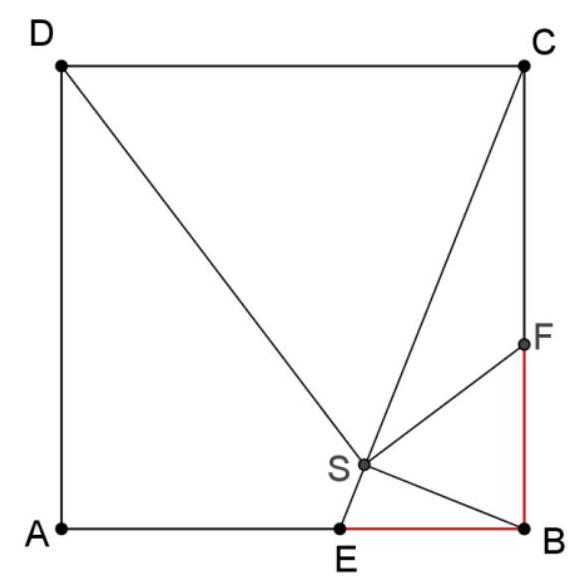
\includegraphics[max width=\textwidth, center]{2024_11_21_0730e5d305676e2c9de1g-1}
\end{enumerate}

\end{document}